
\subsection{Deepfake}
Deepfakes are AI-generated videos or images that convincingly replace the likeness of one person with another, often in a realistic and seamless manner. In today's context, deepfakes raise concerns as they can be used to create misleading content, spreading misinformation, and potentially damaging reputations. This technology has become a notable issue in the age of social media, where manipulated visuals can be easily shared.\\
\begin{figure}[htbp]
    \centering
    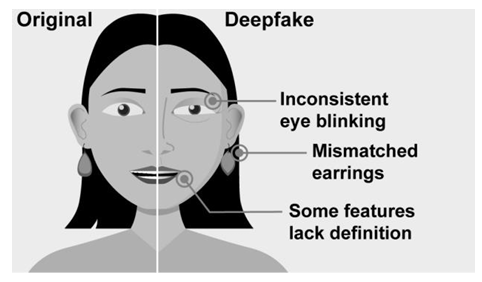
\includegraphics[width=4in]{img/deefakeface.png}
    \caption{{Original vs Deepfakes }}
\end{figure}


\begin{figure}[htbp]
    \centering
    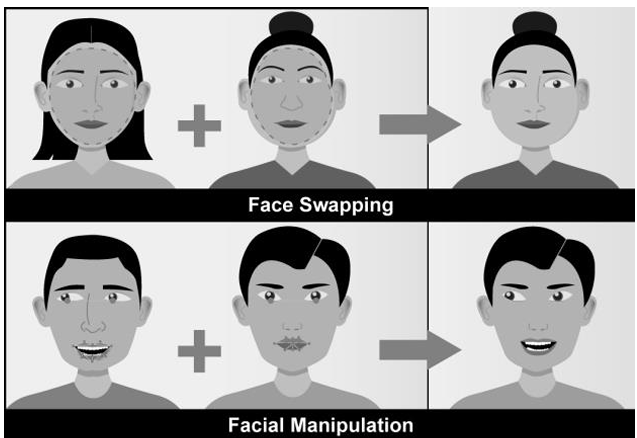
\includegraphics[width=4in]{img/face manipulation.png}
    \caption{{Techniques of Deepfake creation}}
\end{figure}
\noindent Various techniques exist for creating deepfake videos and images, with face swapping and facial manipulation being common methods. Face swapping involves placing the face of one person onto another person's body, while facial manipulation imitates the expressions of one person's face on the face of the target person. Both methods are visually represented in the figure below.\\



